\section*{Aufgabe 1}
\subsection*{a)}
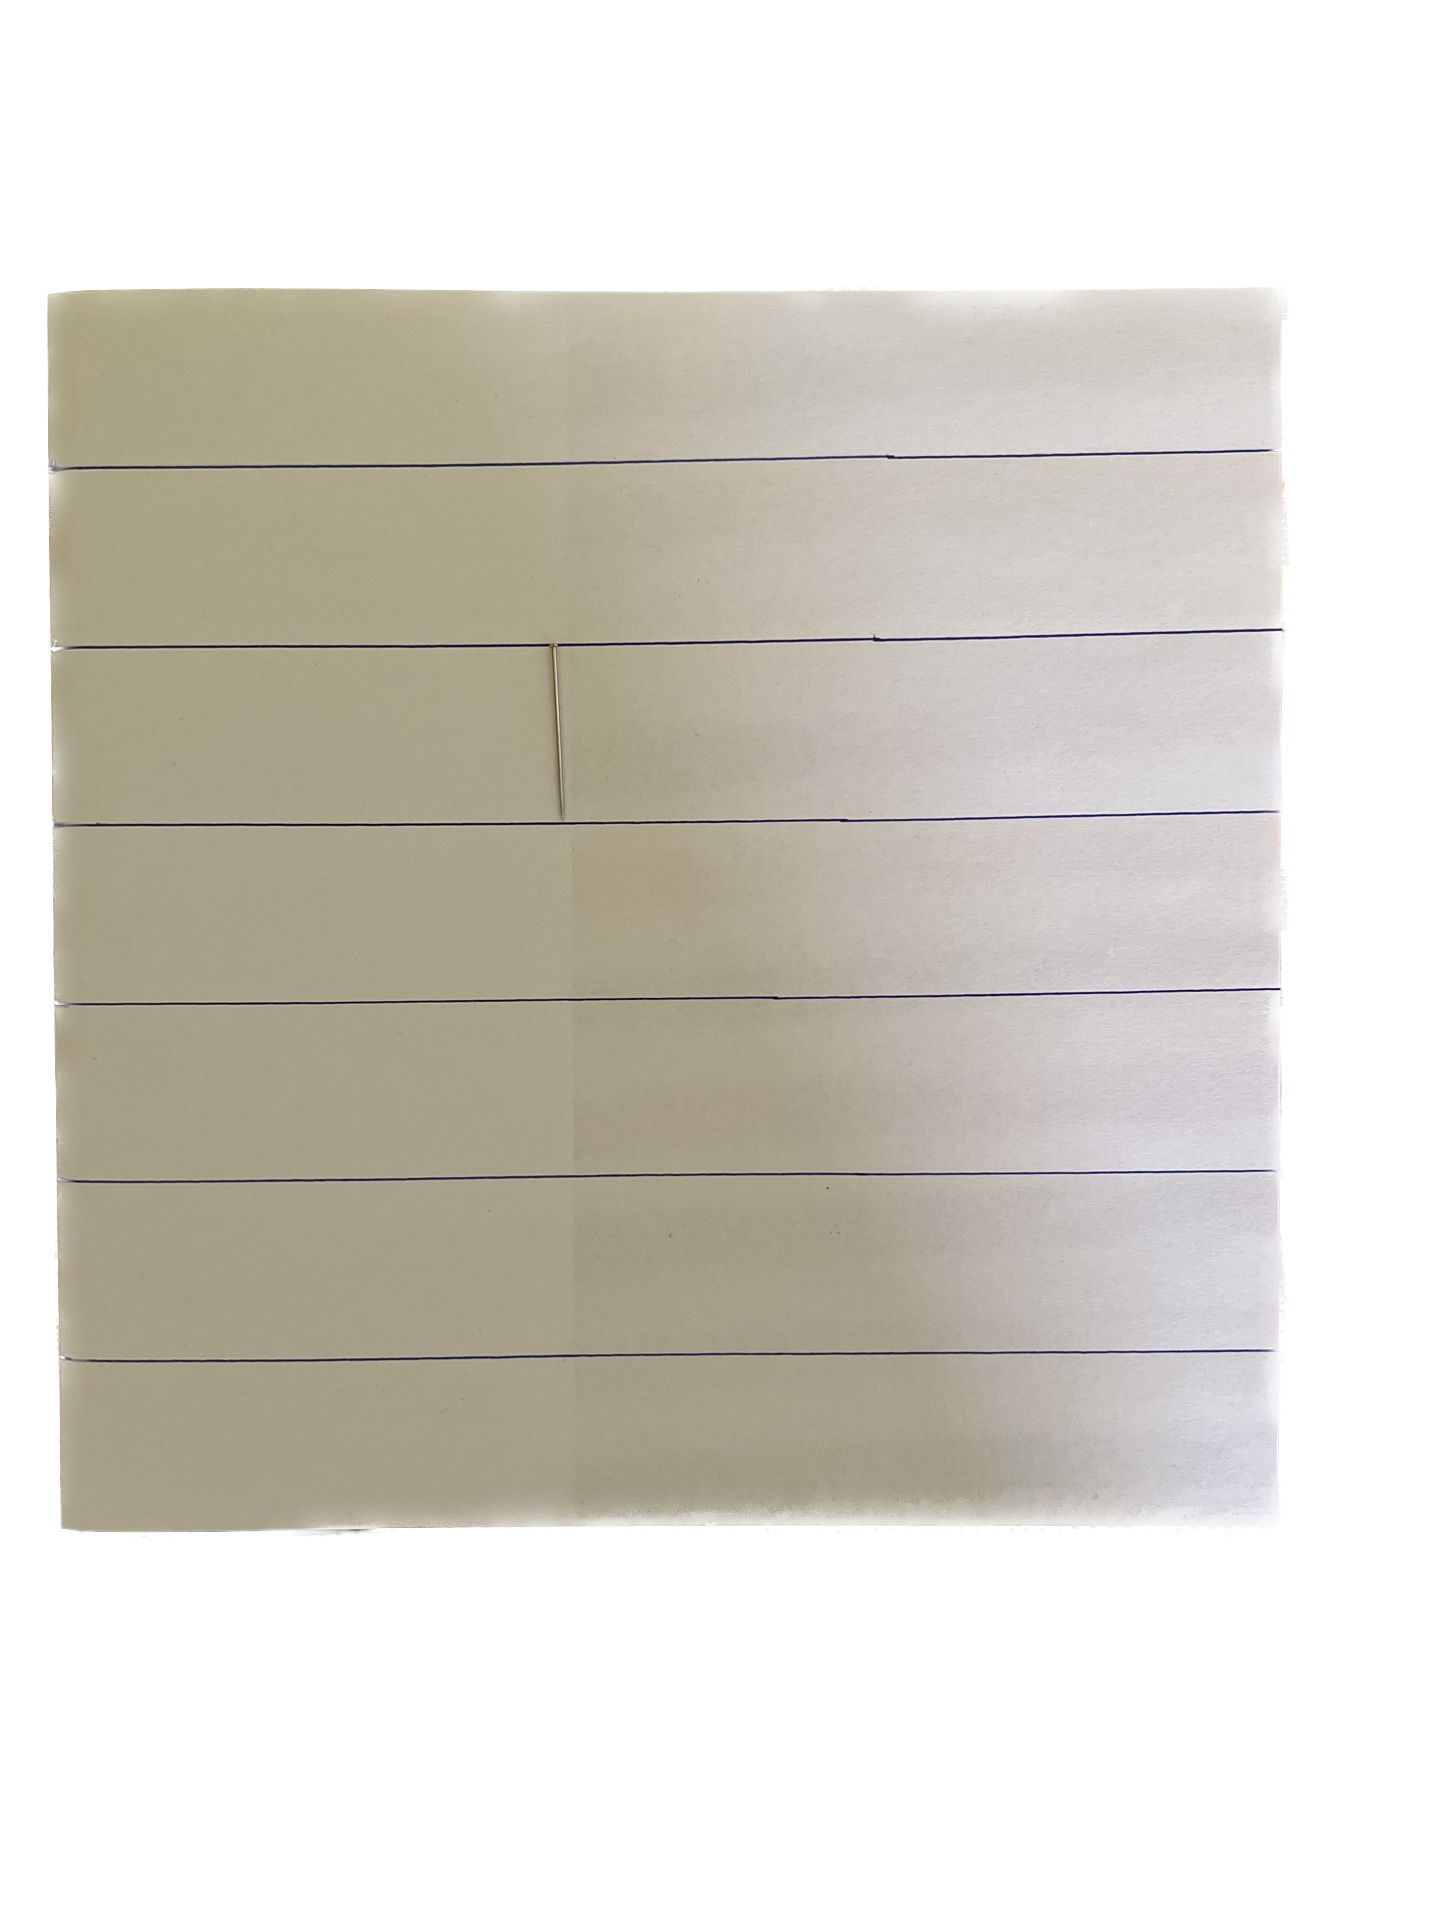
\includegraphics[width=0.8\textwidth]{../img/a1a.png}
\subsection*{b)}
Wie oft die Nadel die Linie schnitt: \textbf{74} \\
Relative häufigkeit: $ \frac{ 74 }{ 100 }  $ \\
Näherung für $ \pi $: $ \frac{ 2 \cdot 100 }{ 74 } \approx 2.703 $
\subsection*{c)}
Die Wahrscheinlichkeit, dass ein zufälliger Punkt im Kreissegment liegt ist die Fläche des Kreissegmentes geteilt durch die Fläche des Quadrates. Also: \\
Fläche des Kreissegments: $ \frac{ \pi }{ 4 }  $\\
Fläche des Quadrates: $ 1 $ \\
$ \rightarrow  $ Wahrscheinlichkeit: $ \frac{ \pi }{ 4 }  $ \\ \\
Um nun $ \pi $ zu approximieren berechnen wir die relative Häufigkeit $ \frac{ T }{ N } $ und lösen nach $ \pi $ auf: \\
\begin{align*}
\frac{ T }{ N } &= \frac{ \pi }{ 4 } \\
\pi &= 4 \cdot \frac{ T }{ N } \\
\end{align*}
\subsection*{d)}
\lstinputlisting[breaklines]{../code/a1d.py}

